%\clearpage
\section{Innovationsmethoden und Innovationsprozesse}
Einleitung.....



\subsection{6-3-5 Methode}\label{subsec:635Methode}
Die 6-3-5 Methode ist eine Kreativitätstechnik zur Ideenfindung, optimalerweise wird Sie in einem Team mit 6 Personen angewendet. Es können Vorideen entstehen, wie auch gezielte Ideeanareicherung entwickelt werden.
\subsubsection{Vorgehensweise}
- In einem ersten Schritt werden Blätter in Papierform, jedem Teilenehmer verteilt, auf denen eine Tabelle mit 3 Spalten und die zuvor definierte Frage enthalten ist. Aus praktischen gründen sollten sich die Teilnehmer am selben Tisch befinden.\\
- Im zweiten Schritt sollte jeder Teilnehmer 3 Ideen zur Grundfrage, also meist eine Lösung für das definierte Problem, in je eine Spalte notieren. Die zeit zum nachdenken ist begrenzt auf 3 Minuten.\\
- In einem weiteren Schritt werden die Tabellen weitergegeben und die jeweils zuoberst beschriebenen Ideen können weiterentwickelt werden. Dieser Schritt wird im gesamten 5 mal durchgeführt.
\subsubsection{Vor- und Nachteile}
\begin{tabular}{|l|l|}
	\hline 
	\textbf{Vorteile} & \textbf{Nachteile} \\ 
	\hline 
	Jeder Teilnehmer kann seine Ideen & Keine Zeit für Fragen  \\
	 Notieren, keine dominanten Personen&\\ 
	\hline 
	Somit ist ein Protokoll erfasst&Es können Redundanzen entstehen \\ 
	\hline 
	Es entstehen in kurzer Zeit sehr viele&Arbeitstakt nicht für jeden Teilnehmer gleich\\
	interdisziplinäre Ideen&  \\ 
	\hline 
	Unnötige Diskussionen entfallen&Braucht eine Vorbereitung \\ 
	\hline 
	Jeder Teilnehmer muss sich beteiligen&  \\ 
	\hline 
\end{tabular} 
\subsubsection{Beispiel}
\begin{figure}[H]
	\centering
	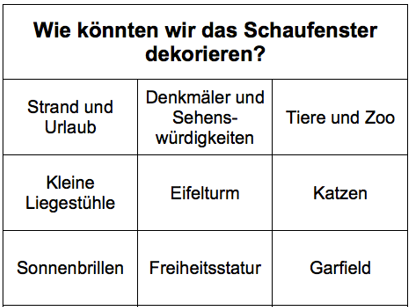
\includegraphics[width=0.5\textwidth]{M635.png}
	\caption{In dieser Abbildung kann erkannt werden, wie Ideen zur Frage: dekoration des Schafensters, entstanden sind}
	%\cite{thirah_vorhangeschloss-schlussel-computer-icons_nodate}
	%\raggedleft
\end{figure}
\newpage
\subsection{Brainstorming}\label{subsec:Brainstorming}

Eine sehr bewährte Variante der Ideenfindung stellt das Brainstorming dar. Hauptsächlich geht es darum aus möglichst vielen Ideen die besten Ergebnisse heraus zu filtern und zu kombinieren. Brainstorming wird am besten in kleineren Gruppen durchgeführt. Wird es in grösseren Gruppen durchgeführt, so entsteht schnell Chaos.

\subsubsection{Vorgehensweise}

- In einem ersten Schritt wird ein Moderator erwählt, welcher die Ideen zusammenträgt und diese für alle sichtbar aufschreibt. Alternativ kann auch eine Wandtafel benutzt werden, auf welche jeder seine Ideen aufschreiben kann.\\
- In einem zweiten Schritt werden Ideen gesammelt. Dabei kann jeder seine Ideen in einer offenen Runde frei dem Moderator mitteilen oder auf die Tafel schreiben. Dies gewährleistet, dass aus bereits genannten Ideen auch neue Ideen entstehen können. Ein wichtiger Punkt dabei ist, dass keine Idee zu abwegig ist. \\
- In einem letzten Schritt werden dann die Ideen sortiert und ausgewertet. Die Teilnehmer sortieren gemeinsam die Ideen und filtern die besten Ideen heraus. Aus diesen Ideen entsteht dann die Zielidee. 

\subsubsection{Vor- und Nachteile}

\begin{tabular}{|l|l|}
	\hline 
	\textbf{Vorteile} & \textbf{Nachteile} \\ 
	\hline 
	Frei Kreativität für jeden & Schwierige Handabung für den Moderator  \\
	\hline 
	Schnelle Ideenfindung & Potential für zu viel input \\ 
	\hline 
	Einbezug aller anwesenden Teilnehmer & Belustigung einzelner bei \flqq abwegigen\frqq  Ideen\\
	\hline
\end{tabular} 


\begin{figure}[h!]
	\centering
	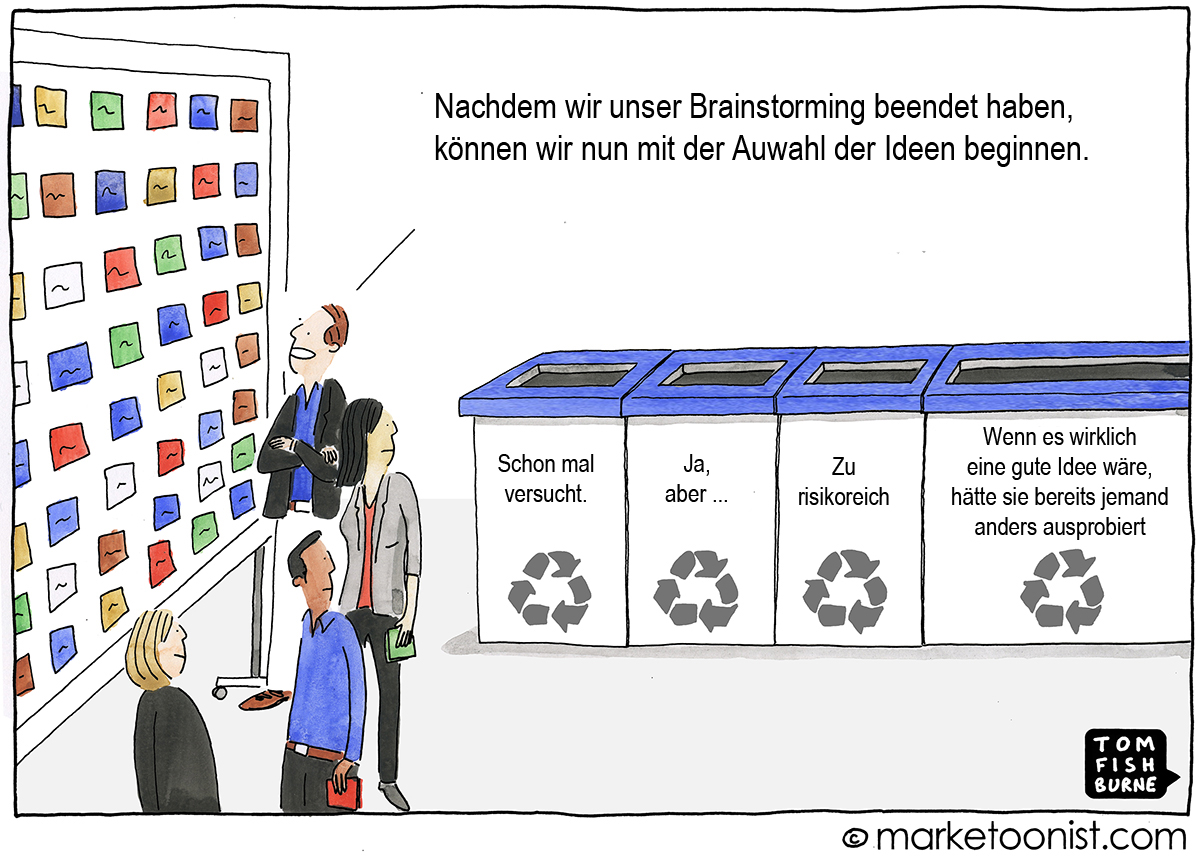
\includegraphics[width=0.8\textwidth]{graphics/Brain}
	\caption{Anschauungsbild Brainstorming}
	\label{fig:Brainstorming}
\end{figure} 




  

